\documentclass{article}
\usepackage[utf8]{inputenc}
\usepackage{graphicx}
\usepackage{adjustbox}

\title{Website ER Diagram}
\date{October 2020}

% ------------
% DOCUMENT
% ------------
\begin{document}
    \begin{flushright}
        CSE 321 Website Storyboard
    \end{flushright}
    
    \begin{enumerate}
        \item[\textbf{Theme}:]
        Ice Breakr - A dating website that puts the conversation first.\\
    
        \item[\textbf{Group Name}:]
        Dream Machine\\
        Group #9\\
    
        \item[\textbf{Members}:]
        Logan Decker, Pierce Mayadag, Wesley Pick-Roth\\
    
        \section{Background}
        \paragraph{}
        When comparing the experiences of each members with websites and apps that we felt could use improvements, we determined that many dating sites tend to have similar problems that the conversations don't go anywhere, or that people feel shallow scrolling through and judging others based on their looks. So we decided to dedicate ourselves to creating a dating site that puts meaningful conversation and connection first, and people can gradually unlock additional interests and information as they talk more.\\
        \section{Website Analysis}
        \subsection{Relevant Websites}
        \paragraph{}
            :Most standard dating websites require users to create a profile by filling out personal information which will then be used to match that user with another user that has related interests and characteristics.
            \begin{enumerate}
                \item[Tinder -]
                A quick and easy-to-use dating site with a focus on more immediate relationships and a minimal design.\\
                
                \item[Bumble -]
                A dating site where women make the first move. Focuses on user initiative by letting users choose the exact kind of relationship they want.\\
                
                \item[Hinge -]
                A dating site where the emphasis is on the user profiles. Tries to make long-lasting matches.\\
                
                \item[Plenty of Fish -]
                A typical dating site. Doesn't really try to focus in on anything.\\
                
                \item[OkCupid -]
                A dating site where matching is highly user-driven (users can look for very specific traits in partners).\\
            \end{enumerate}
        
        \subsection{Desired Features}
        \paragraph{}
        Users must 'unlock' information about a matching user by doing things like having a conversation in order to see user photos. Users will need to enter their location so as to try and match them with other users that are nearby. Users should be shown other potential matches one-at-a-time to try and avoid overloading the user with information. Users will need to enter the kind of relationship that they're looking for in order to better match them, for example, "looking for a short term relationship" or "looking for a lifelong partner". Users will need to fill out the answers to several questions in order to better match them, such as "What job do you have?" or "What do you like to do in your free time?". Our site will filter potential matches with user-specified age and distance filters, and, on the back end, match users with shared interests and information. Users will need to come up with topics of conversation or conversation starters that they find important so as to promote the initial conversation in a match.\\
    \end{enumerate}
    \subsection{Website Feature Comparison}
    \hspace{-2cm}\begin{tabular}{|l|c|c|c|c|c|c|}
        \hline
         & IceBreakr & Tinder & Bumble & Hinge & Plenty of Fish & OkCupid \\
         \hline
         Location of Users & V- & X & X & X & X & X \\
         \hline
         Swipe-Matching & V & X & X & X & X & O \\
         \hline
         Relationship Categories & V & O & X+ & O & X & X+ \\
         \hline
         Personal Information Prompting & V & O & X & X & X & O \\
         \hline
         Unlocking Information & V+ & O & O & O & X & O \\
         \hline
         Filtering & V- & X & X+ & X+ & X & X+ \\
         \hline
         Interest Matching & V+ & X & O & O & X & X \\
         \hline
         Conversation Starters & V+ & X- & X & X & X & X \\
         \hline
    \end{tabular}
    X+: Function included well/focus placed on function\\
    X: Function included\\
    X-: Function included poorly/little focus placed on function\\
    O: Function not included\\
    V-: Function desired but not prioritized\\
    V: Function desired\\
    V+: Function desired and given priority\\
    \section{Storyboard}
    \begin{enumerate}
        \subsection{Potential Users}
        \paragraph{}
        \textbf{Registered users} are users who have already created a profile on our site. After logging in, they will have full access to the site, which includes: uploading profile info, matching with other users, and messaging other users.\\
        \textbf{Unregistered users} are users who do not have a profile on our site. They are restricted to previewing random user profiles or becoming a registered user\\\\
        
        \subsection{Stories & Storyboard}
        \paragraph{}
        All users will start on the "home/login" page. The storyboard we've created is valid for all devices, as smaller screens (like phones) will display the same information in the same format, just with a smaller scaling. Unregistered users will be able to see a sample profile on the landing page to get an idea of what to expect from the website. From there, they can create an account where they'll fill out personal information. Once finished with account creation, they're redirected into the use-case scenario for registered users. For registered users, after logging in, they'll be taken to their own profile's page. Here, users can fill out additional information about themselves, or navigate to the "find matches" page or "messaging" page. Users may also manage their photos, which is its own page that allows users to upload, delete, and rearrange their photos. From any main page, users may navigate to their own profile, the messaging page, the matching page (all by using the buttons at the top of the page), and the landing page (by logging out). The "find matches" page will present the user with information about a different user and they will be prompted to accept or reject the match. The "messaging" page allows the user and any matches to message each other, as well as access the other users' profiles, which are identical to the personal profile except that some information is hidden until conversational benchmarks are met. The user storyboards are included in the "storyboard.pdf" file.
    \end{enumerate}
    
    \begin{enumerate}
        \section{Database Design}
        \subsection{ER Diagram}
        The ER Diagram that follows allows us to visualize the way the database is going to be organized and implemented. It also highlights the relationship between different elements in our database\\
        $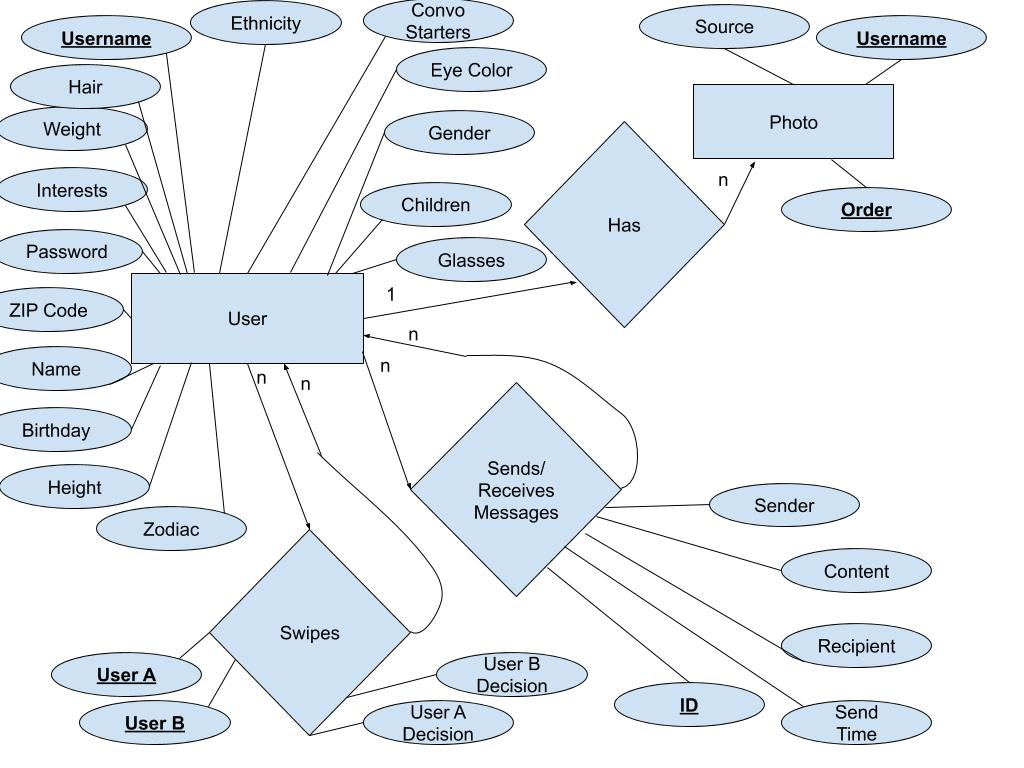
\includegraphics[width=0.9\columnwidth]{ERDiagram.jpg}$\\\\
        
        \subsection{Table Design}
        \textbf{User Table}\\
        \begin{adjustbox}{width=1.2\textwidth}
            \begin{tabular}{|c|c|c|c|c|c|c|c|}
                \hline
                Primary Key & Field Name & Data Type & Non-Null & Unique & Binary & Foreign Key & Comments \\ \hline
                X & Username & varchar(32) & X & X &  & X & Identifies each user\\ \hline
                 & Password & varchar(32) & X &  &  &  & User's password\\ \hline
                 & Name & varchar(32) & X &  &  &  & User's real name\\ \hline
                 & Birthday & datetime & X &  &  &  & User's birth date\\ \hline
                 & Gender & uint(1) & X &  &  &  & User's gender (each value 0-9 corresponds to a list value)\\ \hline
                 & ZipCode & uint(5) & X &  &  &  & User's zip code\\ \hline
                 & HobbiesInterests & varchar(16) & X &  &  &  & Each bit corresponds to an interest (A 1 indicates an interest while a 0 indicates no interest)\\ \hline
                 & ConversationStarters & varchar(512) & X &  &  &  & Topics the user can talk about\\ \hline
                 & Height & uint(2) &  &  &  &  & User's total height in inches\\ \hline
                 & HairColor & uint(2) &  &  &  &  & User's hair color (each value 0-99 corresponds to a list value)\\ \hline
                 & ZodiacSign & uint(2) &  &  &  &  & User's zodiac sign (each value 0-99 corresponds to a list value)\\ \hline
                 & Children & uint(2) &  &  &  &  & Number of children the user has\\ \hline
                 & Weight & uint(3) &  &  &  &  & User's weight in pounds\\ \hline
                 & EyeColor & uint(1) &  &  &  &  & User's eye color (each value 0-9 corresponds to a list value)\\ \hline
                 & Ethnicity & varchar(32) &  &  &  &  & User's ethnicity\\ \hline
                 & Glasses & uint(1) &  &  & X &  & Whether or not the user wears glasses (0 if no, 1 if yes)\\ \hline
            \end{tabular}\\\\
            
        \end{adjustbox}\\
        This table holds all of the user's information. Each user has a unique username, and a password that they use to log into their account. They also have a lot of personal information. Most information is stored as a character string. The fields that aren't strings are stored as integers that correspond to values in lists. The idea is that users will select an option from a pre-determined list, and we store the position in that list. The hobbies/interests field is stored as a bit string, where each character in the string corresponds to a different hobby/interest. A 1 in that position indicates that the user has that hobby/interest, while a 0 indicates that the user does \textbf{not} have that hobby/interest. The date of the user's birth is stored as a datetime corresponding to midday of their birthday.\\
        The username must be unique, and, as such, is used for all other tables. By using the username as a foreign key, we can identify which user a Photo or Message belongs to, or whether or not they Swipe yay/nay on another user.\\\\
        
        \textbf{Photo Table}\\
        \begin{adjustbox}{width=1.2\textwidth}
            \begin{tabular}{|c|c|c|c|c|c|c|c|}
                \hline
                Primary Key & Field Name & Data Type & Non-Null & Unique & Binary & Foreign Key & Comments \\ \hline
                X & Username & varchar(32) & X & X &  & X & Identifies this photo's user\\ \hline
                X & Order & uint(1) & X & X &  &  & Determines position of this photo compared to others\\ \hline
                 & Source & varchar(256) &  &  &  &  & Photo's URL\\ \hline
            \end{tabular}
        \end{adjustbox}\\\\
        This table holds the information for a user's photos. Each user is allowed to have up to 9 photos. Each photo has a corresponding user and order (1-9) where a lower order means that it's displayed sooner. A value of 0 in the order means that the photo does not exist, which will occur if a user only has 8 or fewer photos. The source is the URL where the photo is uploaded. We'll use this URL to load the photo on our site.\\
        The username is used for all other tables. By using the username as a foreign key, we can identify which user these photos belong to.\\\\
        
        \textbf{Swipe Table}\\
        \begin{adjustbox}{width=1.2\textwidth}
            \begin{tabular}{|c|c|c|c|c|c|c|c|}
                \hline
                Primary Key & Field Name & Data Type & Non-Null & Unique & Binary & Foreign Key & Comments \\ \hline
                X & UserA & varchar(32) & X & X &  & X & Identifies first user of matching pair\\ \hline
                X & UserB & varchar(32) & X & X &  & X & Identifies second user of matching pair\\ \hline
                 & UserADecision & uint(1) &  &  & X &  & First user's swipe decision\\ \hline
                 & UserBDecision & uint(1) &  &  & X &  & Second user's swipe decision\\ \hline
            \end{tabular}
        \end{adjustbox}\\\\
        This table determines if two users are a match for each other. Each time a user swipes another user, if a table involving these two users doesn't already exist, a new one is created. The first user to swipe the other corresponds to UserA, and their decision is stored in UserADecision (0 if 'nay' and 1 if 'yay'). When the first user then shows up for the potential match, the second user and their decision are stored as UserB and UserBDecision. If both fields are 1s, it's a match! These two users may then start sending each other messages. While a user is undecided, their Decision field remains null.\\
        The two usernames are used to form the primary key for each match. Each username is a foreign key that corresponds to two different users that compose the match.\\\\
        
        \textbf{Message Table}\\
        \begin{adjustbox}{width=1.2\textwidth}
            \begin{tabular}{|c|c|c|c|c|c|c|c|}
                \hline
                Primary Key & Field Name & Data Type & Non-Null & Unique & Binary & Foreign Key & Comments \\ \hline
                X & ID & uint(8) & X & X &  &  & Identifies the specific message\\ \hline
                 & Sender & varchar(32) & X &  &  & X & Username of this message's sender\\ \hline
                 & Receiver & varchar(32) & X &  &  & X & Username of this message's recipient\\ \hline
                 & Content & varchar(512) & X &  &  &  & Content of the message\\ \hline
                 & TimeSent & datetime & X &  &  &  & Time at which this message was sent\\ \hline
            \end{tabular}
        \end{adjustbox}\\\\
        This table holds all the information for a message that one user sends to a matching user. The message ID is a unique 8-digit number that identifies this specific message. The sender and recipient are the users that this message is being sent between. The content contains the actual text of the message, and the time the message was sent is stored in TimeSent as a datetime. The TimeSent field will be used to sort the display of the messages.\\
        The two usernames are foreign keys that correspond to two different users that are messaging each other.\\
    \end{enumerate}
    \section{System Architecture}
    $\includegraphics[width=0.9\columnwidth]{"SystemArchitecture.png"}$\\
    \begin{enumerate}
         \textbf{The User class} stores all of a user's information (username, real name, gender, birthday, etc) as well as methods for getting and setting all of that data. It also contains some methods for generating special content, like Zodiac signs from the birthday.\\
         \textbf{The Pictures class} stores the URLs of all the photos of a user, as well as ways to get and set them. It also keeps track of how many photos the user has uploaded, which it updates using a special method.\\
        \textbf{The SwipeQueue class} contains a queue of the next profiles (up to 16 profiles) that the current user will see as they make selections on the match page. When a user makes a selection (Yay or Nay) that profile is removed from the queue. When the queue is empty, it will load the next 16 profiles from the data base. Profiles are selected by 4 criteria: 1. Gender preference compatibility, 2. Whether or not the current user has already seen the profile in the match page, 3. Whether or not the other profile's user has already seen the current user's profile in their match page, and 4. Number of Interests the two profiles have in common.\\
        \textbf{The CredentialError} class keeps track of input errors for the login and registration process. If a user submits a non-valid username when logging in, or an unavailable username when registering, the NameErr field is set. If a user submits an incorrect password when logging in or their password doesn't match the re-entered password when signing up, the PassErr field is set. If a user submits an incomplete registration form, (1 or more required fields are empty), the EmptyErr field is set.\\
        \textbf{The Conversations class} stores all of the user data that a user can have a conversation with based on the information in the database from their swipe history. It also stores information about a current user for the messaging feature to figure out who is being talked to.\\
        \textbf{The Messages class} stores the conversation history between users. This is stored between the contents of the message, as well as who the sender and receiver of each message is.\\
        \textbf{The Servlet class} contains all of the logic for navigating between the pages as well as calls to the database for updating and receiving information. Depending on the action that it receives, it may load a new page, populate User and Pictures classes, update information in the database, pull information from the database, or more.\\
        \textbf{The Profile, Other Profile, and Preview Profile jsp files} display information from a User and a Pictures that the Servlet creates. The Profile file specifically also sends information to the Servlet for updating any user information, which updates the database. The Other Profile file check the User's Icebreakr Score before displaying some of the information. If the score isn't high enough, the information will be hidden. Increasing the score is done from the Servlet while sending messages. Preview Profile will never display fields that can be hidden and therefore doesn't ever use a Pictures class at all. Profile is accessed from Index, Conversation, Match, Other Profile, Pictures, and Signup. Other Profile is only accessed from Conversation. Preview Profile is accessed only from Index.\\
        The Pictures jsp file displays all photos that the logged-in user has (which are populated via the Servlet) and also sends updated URL information to the Servlet so that the Photo database can be updated. Pictures is only accessed from Profile.\\
        \textbf{The Index jsp file} is the login page and also the landing page of the website. From here, user have three options. They can login with an existing account, (success directs to profile page, failure results in error). They can register a new account, (redirects to signup page). They can also preview the profile of a randomly chosen member.\\
        \textbf{The Signup jsp file} is where a user can register a new account. Here a user inputs all the essential information for creating a new profile, (username, password, name, birthday, location, gender, gender preference, interests, and conversation starters). If the entered username is not already taken, the password field matches the re-entered password field, and no fields are left blank, then submitting the form will create a new entry in the User table of our database. In addition to this, one new entry in the Swipe table of our database is made for every other existing user. If the submitted username is taken, passwords do not match, or if any fields are left empty, then the user receives the corresponding error.\\
        \textbf{The Match jsp file} displays the next profile in the current user's swipe queue and allows them to decide whether or not they like that profile (Yay or Nay). When the current user makes a selection on a profile, the row in the swipe table of our data base that corresponds to the current user and the profile they viewed is updated. Then, the profile they viewed is removed from their swipe queue and they are presented with the next profile in their swipe queue.\\
        \textbf{The Conversations jsp file} displays all users that a user can have a conversation with on the left side. When a user is selected, it retrieves the conversation history between them and displays all sent messages between them in order of where they were sent. The messages are distinguished with different colors and positions depending on who was the sender and who was the receiver of the message. It also allows you to click a button to access that specific user's profile page.
    \end{enumerate}
    \section{System Snapshot}
    \section{Conclusion}
    $\includegraphics[width=0.9\columnwidth]{"login-preview.jpg"}$\\
    Roberto wants to make an account in Icebreakr and see what the website has to offer for him. He goes to the website URL and arrives at the landing page. He is prompted to login with a username and password, however he does not currently have an account. There is a hyperlink lower down that tells him that he can register a new account if he is a new user. He can also see that he has the option to “Preview Member”, so he decides to click that to get a taste of the website before he dives in.\\\\
    $\includegraphics[width=0.9\columnwidth]{"preview.jpg"}$\\
    After clicking “Preview User”, Roberto can see the profile information of someone named “Tot”. He can see some basic information, like that they are apparently 7 years old and like art and gardening. However, other pieces of information like their height and ethnicity are hidden behind question marks. This is because Roberto is not viewing this with an account, so some profile information is not revealed. With nowhere else left to go (except another website, but Roberto is hooked so he’s not going to leave), Roberto clicks “Back To Login” to take him back to the login page.\\\\
    $\includegraphics[width=0.9\columnwidth]{"login-register.jpg"}$\\
    Roberto is now confident that he wants to register a new account, as he does not own one currently, so he clicks “Register new account!”\\\\
    $\includegraphics[width=0.9\columnwidth]{"register.jpg"}$\\
    Roberto is taken to a page where he can enter in personal details about himself for the website. From his prior knowledge, he can see a lot of the information he is prompted to give here is what is publicly displayed from the user he saw after clicking the “Preview Member” button earlier. He fills in each field with answers that are true to himself or that he thinks are appropriate. He creates a username and password, enters his name, birthday, and location in the appropriate fields, then specifies his gender and what types of people he is interested in meeting on the dating site. He then selects the checkboxes for activities he considers to be appropriate hobbies or interests in his life. Finally, he fills in a phrase or so that he hopes can get an engaging conversation started with him. When he is finished, he clicks “Register” to finish making his account.\\\\
    $\includegraphics[width=0.9\columnwidth]{"profile.jpg"}$\\
    Roberto is brought to his profile. The information he displayed at registration is shown to him, but some of the fields also give him the option of changing them or adding additional information.\\\\
    $\includegraphics[width=0.9\columnwidth]{"updating-profile.jpg"}$\\
    Roberto begins to fill in more information about himself in all of the categories, including re-stating some of the information he already entered before, and then clicks on “Update Profile” to commit the changes.\\\\
    $\includegraphics[width=0.9\columnwidth]{"profile-manage-pictures.jpg"}$\\
    Roberto is still on his profile page, but now the information that is entered about himself has changed to match what he had entered before clicking the “Update Profile” button. He wants to add some images of himself to his profile while he’s already in the process of creating his profile. So he clicks on the “Manage Pictures” button.\\\\
    $\includegraphics[width=0.9\columnwidth]{"photos.jpg"}$\\
    On the manage pictures button, Roberto is told of the instructions of how it works. Roberto then finds a couple of URLs for images that he thinks would be appropriate representations of him and places them in the first and second text boxes. He then clicks “Finish Changes” to set those images as his first two images on his profile.\\\\
    $\includegraphics[width=0.9\columnwidth]{"updated-profile.jpg"}$\\
    Roberto is brought back to his profile page, where his first image is now being displayed on his profile alongside the other information he entered earlier. With that, he is ready to begin trying to meet new people and clicks on “Start Matching!”\\\\
    $\includegraphics[width=0.9\columnwidth]{"match.jpg"}$\\
    He is brought to the matching page, where the information about a user named “Gina” is being displayed to him. He can see her age, gender, location, hobbies/interests, and conversation starter that she entered when she created or updated her profile. Roberto thinks she seems like a nice person and clicks “Yay!” to show his approval. After he does this, a new user’s information is displayed to him. With this approval and disapproval process, he continues to click “Yay!” or “Nay!” on a few more people presented to him. Once he gets bored, he clicks on “Conversations” to see if anyone he expressed “Yay!” to did the same for his profile.\\\\
    $\includegraphics[width=0.9\columnwidth]{"conversations1.jpg"}$\\
    Roberto is brought to his conversations page, where he sees that Gina, who he said “Yay!” to earlier, now appears on the left side. He clicks on her name to see their message history, and he can see that she has sent a message to him. To respond, he types in a message to her and clicks “Update” to send the message he typed to her. He then clicks on her name above the conversation history to take a look at her profile.\\\\
    $\includegraphics[width=0.9\columnwidth]{"other-profile1.jpg"}$\\
    Now Roberto can see Gina’s profile page. It shows some information about her but continues to hide some parts of her profile from him since they have not talked enough yet. Roberto then commits to talking with Gina more to get to know her and clicks on “Conversations”.\\\\
    $\includegraphics[width=0.9\columnwidth]{"conversations2.jpg"}$\\
    Roberto then repeats the process of typing messages and clicking “Update” to send his messages to Gina. Eventually, Gina responds to his message and he can see their full conversation history. With this, Roberto clicks on her name above the conversation history again to see if any more information on her profile has been revealed.\\\\
    $\includegraphics[width=0.9\columnwidth]{"other-profile2.jpg"}$\\
    Now that he has a longer conversation history with Gina, Roberto can see more hidden parts of her profile, such as her height and the first image that she uploaded to her profile. Satisfied to learn more about Gina and start a new friendship, Roberto clicks on “Logout” to conclude his use of the website.\\\\
    $\includegraphics[width=0.9\columnwidth]{"login.jpg"}$\\
    After logging out, Roberto is brought back to the landing page with his browser session no longer holding onto his login information. He is now fully safe to leave the website.\\\\
    \subsection{Accomplishments}
    \paragraph{}
    In our final implementation of the website, we accomplished nearly all goals we set out to achieve.
    \begin{itemize}
    \item We created a functioning login and registration page, as well as the database back-end to store user profile information.
    \item We implemented the preview user function for unregistered users.
    \itemThe user profile page displays the users information and allows them to update non-permanent fields.
    \item The user matching function is fully functional, featuring a a queue of user profiles prioritized by gender preference, swipe history, and common interests.
    \item The swipe tables for all users are correctly updated and retrieved from the database.
    \itemThe conversation page is functional, allowing users to send messages to users they've matched with and also view their profiles.
    \item The message history for all users is correctly updated and retrieved from the database.
    \item Viewing other user profiles from the conversation page correctly display their information and a primitive version of the Icebreakr algorithm was implemented. (The Icebreakr algorithm hides certain information and pictures on a user's profile page until you have attained a certain threshold of conversation with that user)
    \end{itemize}
    \subsection{Future Work}
    \paragraph{}
    Although we accomplished nearly all of the goals we set for our website, there were a couple notable features that were left out.
    \paragraph{}First off were the pictures. Image files themselves were never capable of being uploaded to the database, the database simply stores the URL of images. This means that only pictures with an existing URL on the internet could be uploaded. Furthermore, displaying the pictures uploaded in this manner was not functional in the final version of the website, although it was in previous versions.
    \paragraph{}
    The other major goal we fell short of was the Icebreakr algorithm. This was the algorithm that allowed users to gradually unlock information and pictures about others through conversation. Although a primitive version of the Icebreakr algorithm was implemented, it simply concealed all additional user information until one message had been sent by each user.
    \paragraph{}
    One small feature missing from our conversation page was the ability to remove conversations with other users, there by unmatching with that particular user.
    \paragraph{}
    One notable vulnerability in our website was with the date of birth field in our sign-up page. For one thing, the field for entering date of birth allowed erroneous dates such as February 31st. Furthermore the upper limit on the year, month, and day fields were only enforced by built in JavaScript, so disabling JavaScript would allow further erroneous input. The solution to this would be to error check the fields corresponding to the date of birth before submitting the update request to the database.
    \paragraph{}
    Lastly, the visual design of our website was passable, but not aesthetically pleasing, especially in comparison to many modern websites. Although this was never a goal of ours, it would be worth investing time into for future work.
\end{document}